This section presents an explanation on the design of the solution from a technical point of view and the reasons behind it. Its main points are the description of its architecture, followed by an explanation of the framework and the technologies which the implementation is based on, the reasons for it, and the pros and cons of the solution, as well as a more detailed insight on several aspects of the project development and workflow, such as testing, data persistence, deployment and the overall infrastructure.

\section{Why an API?}
Using an API as the core of the solution allows a decoupling that is key to the idea of the whole project. The API will provide access to the business logic in modular ways, giving the potential clients plenty of possibilities to develop or use different features according to their needs.

With libraries like ReactJS, Angular and other similar frameworks it makes sense to provide a backend platform fully decoupled from any frontend. The backend provides the business logic while the frontend decides and defines how the interaction with the user works. Taking this into account, the API is designed with the intention to provide low level decoupled interactions the complete the business logic but don’t condition the interaction with any of them.

In order to further explain this idea, there is a very direct example in the platform that can be used to depict a probable situation. There are two endpoints on the API that are used for increasing or decreasing the stock of a product. At the conceptual level, these endpoints are closely related to buying from a provider (and thus increasing the stock) and selling products to a customer (and thus decreasing it). While it could make sense to have this logic directly coupled to endpoints related to buying or selling orders, having these logics separated, although meaning some extra work in other fronts, makes it easier for different clients with different needs to use these endpoints through their own custom buying and selling logics.

\section{Architecture}
Following is a high-level diagram of the overall architecture for the solution with a general explanation of each of its parts.

\includegraphics[width=\textwidth]{oa.png}

For this particular instance, the app (the API backend) is hosted and run in a dedicated server. The database is also hosted in the same server. This server is managed through and administrator interface. Throughout the development of the project the management has been done through SSH from the administrator computer to the hosting server. From this server the API is exposed, and consumed from two different fronts. 

On on side clients in the main server’s LAN can directly access the API. This would mimic having a server in, for example a warehouse that has also POS’s (points of sale), which would be the computers or devices that access through the same LAN or WAN.

On the other side the API is optionally exposed on the internet so it can be accessed from other devices and client applications. An example scenario for this would be to build a read-only mobile application to view reports and business data from the application.

Note that this design is for the demo implementation. The system is built so it can adapt to different architectures. For example, as it is seen in the diagram, the application and the database are stored in the same server. In other instances the database could be hosted in a dedicated server.

\section{Technologies}
The backbone of the project, the API that implements the business logic of the solution, is implemented in PHP 5.5.9. The reason for using this language among others are that it is very agile and straightforward. Although many would argue in favour of other technologies for projects of this type, the previous experience with this language from the people involved and the requirements of the project, such as speed and simplicity of development, make it a good choice.

\section{Laravel}
Laravel is an open source PHP framework created in 2011 by Taylor Otwell as a more advanced and friendly alternative to Codeigniter and other frameworks from the moment. Although in its initial version it did not provide support for controllers, currently it’s a fully MVC (model-view-controller) oriented framework. Its key features start by being friendly, intuitive and clean, making it pretty straightforward to implement basic and simple applications using only features and capabilities provided out-of-the-box by the framework.

That said, Laravel was not the original decision. Instead the intention was to use its lighter sibling, Lumen, a lightweight version of Laravel that includes the very basics. Although using the light version would be a great opportunity for this project, it lacked a key feature that proved very important. At the moment, Lumen did not support routing on subdomains. This was key requisite in the design application, so the decision to trade lightness for this feature, which is supported on the full Laravel framework was direct.

The key points that established the decision to use this framework for this project are, to begin with, the previous knowledge and experience from the people initially involved, which reduces the learning curve and the time to get a working MVP up and running.

Another decisive feature is the ease to jumpstart, install and deploy the application. Having the right knowledge and experience, taking a simple application from zero to a production environment can take a simple matter of hours, while deploying the basic installation of Laravel is a matter of minutes.

From the API development point of view, the routing features provided by Laravel, described more in detail in the following section, are a big plus.

Also Laravel provides a very straightforward and solid authentication system out-of-the-box. This is again described in more detail in a following section.

As with most of the frameworks, Laravel also provides the order and advantages of a defined file structure, as well as a set of helpers that turn common, often tedious tasks into something easy.

Finally, Laravel also comes with a friendly and intuitive templating engine. However this is not something exploited on this project so no further detail besides mention is needed.

\section{Routing}
One of the most powerful features provided by Laravel is its routing engine. Explained in a simple way, routing consists on assigning the different routes an application has (the addresses used) to their different pages, actions, controllers and so on. These routes are defined in the app/http/routes.php file. For an example, following is the most basic example of a route in Laravel, borrowed directly from the \href{https://laravel.com/docs/5.3/routing}{official Laravel documentation}:

\begin{minted}[frame=lines,framesep=2mm,baselinestretch=1.2,bgcolor=lightgray,fontsize=\footnotesize,linenos]{php}
Route::get('foo', function () {
    return 'Hello World';
});
\end{minted}

So if the base URL for the application were to be www.smappapp.com, this route would cause that going to www.smappapp.com/foo would render ‘Hello World’ in the browser. The simplest route, as in the example provided, is therefore a route and a closure (or callback) function. This callback function can be either defined directly in the routes file or referenced from there.

To reference a particular function you can reference directly a whole controller and the function. This is the case for most of the routes of the application of this project, as seen here, with the main definition for the routes used in the Products features:

\begin{minted}[frame=lines,framesep=2mm,baselinestretch=1.2,bgcolor=lightgray,fontsize=\footnotesize,linenos]{php}
// Products
Route::get('products', 'ProductsController@index');
Route::get('products/{id}', 'ProductsController@find');
Route::post('products', 'ProductsController@store');
Route::delete('products/{id}', 'ProductsController@delete');
\end{minted}

(Note this code was extracted at the time of the documentation for the purpose of an example, and could be outdated)

All the routes on the example reference the ProductsController controller, which contains the business logic related to products and answers to all the actions related to them. As it can be deduced, when reading the code for the controller, the methods index, find, store and delete can be found.

As can also be seen with the example, different HTTP method calls are defined on the routes. Laravel automatically manages the differentiation of these calls, so while the route:

\begin{minted}[frame=lines,framesep=2mm,baselinestretch=1.2,bgcolor=lightgray,fontsize=\footnotesize,linenos]{php}
Route::get('products', ...);
\end{minted}

and:

\begin{minted}[frame=lines,framesep=2mm,baselinestretch=1.2,bgcolor=lightgray,fontsize=\footnotesize,linenos]{php}
Route::post('products', ...);
\end{minted}

will essentially look the same, they are routed to different methods and therefore have different behaviours, as they trigger different methods.

\subsection{Grouping}
Laravel’s routing engine also supports grouping routes, which essentially allows to group routes according to a certain criteria. A very explicit use case for this feature in the application is for adding the API prefix to the routes:

\begin{minted}[frame=lines,framesep=2mm,baselinestretch=1.2,bgcolor=lightgray,fontsize=\footnotesize,linenos]{php}
Route::group(['prefix' => 'api/v1', ...], function() {
	//...
}
\end{minted}

This prefix automatically causes all the routes to add \code{'api/v1'} on the beginning of the route. So while defining the following route:

\begin{minted}[frame=lines,framesep=2mm,baselinestretch=1.2,bgcolor=lightgray,fontsize=\footnotesize,linenos]{php}
Route::get('products', ...);
\end{minted}

will define the action or page for \code{\textless some\_url\textgreater/products}, if we add the route to the grouping, the definition will become the one for \code{\textless some\_url\textgreater/api/v1/products}.

This is very useful for managing APIs, particularly their versions, as there could be different groupings, each one with a different prefix defined for every different version, and with routes that point to the pertinent controllers.

\subsection{Middleware}
The next useful feature of Laravel’s routing is the middleware definition. Middlewares are additional layers that provide logic to the routes. Arguably the most used and popular one is the Auth middleware, that provides authentication logic for the applications. Laravel allows the implementation and injection of custom middlewares but also provides some by default, the Auth one becoming native to Laravel from version 5.1 onwards, due to its popularity and widespread use.

The middleware used for the application is auth:api, an authentication layer for API-oriented application. In order to use the middleware it must be added to the routes. In the application it has been done in the grouping for the API calls:

\begin{minted}[frame=lines,framesep=2mm,baselinestretch=1.2,bgcolor=lightgray,fontsize=\footnotesize,linenos]{php}
Route::group([..., 'middleware' => ['auth:api']], function()
	...
}
\end{minted}

There are several pros and cons to this system. The pros are the ease of use and the code simplicity. The cons are simply that the authentication process is transparent to the developer. This means that if the generic method is enough, there is no problem, but introducing variations or additional features and logic can be a problem.

\subsection{Additional features}
Some very useful additional features related to routing in Laravel are the bootstrapped routes, such as Route::auth(); that will automatically, and in a transparent way, generate all the routes needed for an authentication platform, including login, registering capabilities, password recovery, and so on.

And finally, an indirect perk of this system is that the code itself provides a very clear roadmap of the application that is built. This can be seen either by reading the code itself or, for example, running the following command:

\begin{minted}[frame=lines,framesep=2mm,baselinestretch=1.2,bgcolor=lightgray,fontsize=\footnotesize,linenos]{bash}
php artisan route:list
\end{minted}

The output of this command is a table with the current routes that are in place, as seen in the following example:

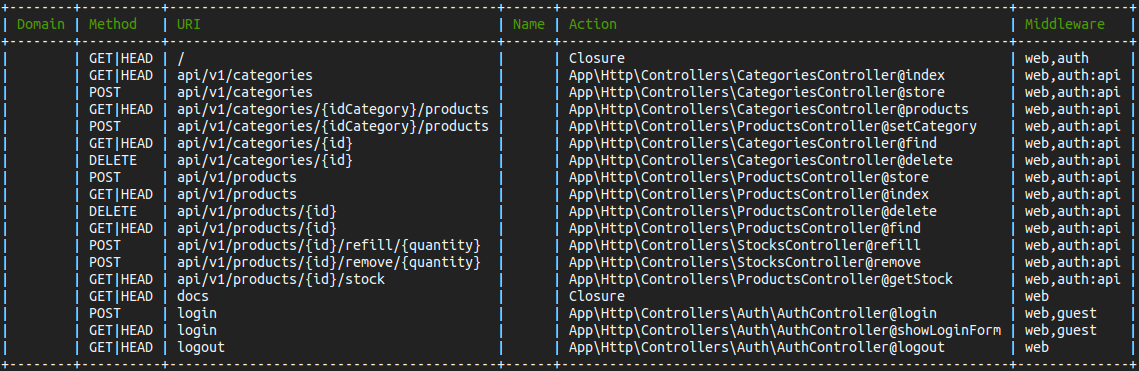
\includegraphics[width=\textwidth]{to.png}

\section{Database}
The database technology of choice for this project is SQLite. There are various reasons for this choice, the most important being the lightness and the simplicity of installation and use. Once the technology is installed, there is no further action required from the user to get it up and running. Although there are several technologies that are often said to be more powerful or reliable for production environments, like PostgreSQL or MySQL, these technologies are slightly more complicated to setup and maintain. Usually SQLite is disregarded for production environments because of its lightness, as if it was a sign of unreliability or the lack of ability to scale. After doing some research, however, there are no reasons to think that SQLite will not perform properly for an architecture and an infrastructure as the one explained in this project.

Taking all this into account, the conclusion is that SQLite offers enough advantages as to be a straightforward decision.

The main advantage of this technology is that the database is basically a single file. That makes it completely standalone and easy to maintain. Backups of the database can consist in merely copying the file to a secure or redundant location. However, if further interaction is required with the database, there are database managers specific to SQLite that can fill this purpose with capabilities like data dumps, data corrections, raw querying, database management and so on.

The native creation, access and management of the database occurs in a transparent way during the installation of the application, and can be done with the default parameters that are already configured in \code{config/database.php} and the \code{.env} file shipped with the standard solution.

The configuration needed for setting up the SQLite database is the following:

\begin{minted}[frame=lines,framesep=2mm,baselinestretch=1.2,bgcolor=lightgray,fontsize=\footnotesize,linenos]{php}
'connections' => [

   'sqlite' => [
       'driver' => 'sqlite',
       'database' => env('DB_DATABASE', database_path('database.sqlite')),
       'prefix' => '',
   ],

],
\end{minted}

This configuration reads the \code{DB\_DATABASE} parameter from the \code{.env} file to set the filename for the database. If the parameter is not found on a \code{.env} file, the default will be \code{database.sqlite} in the \code{/database} folder of the project.

This configuration comes by default with Laravel alongside several other native configurations for different database technologies, specifically MySQL and PgSQL. In order to define SQLite as the technology to be used, it has to be declared as the default with the following line of code, found on the \code{config/database.php} file.

\begin{minted}[frame=lines,framesep=2mm,baselinestretch=1.2,bgcolor=lightgray,fontsize=\footnotesize,linenos]{php}
'default' => env('DB_CONNECTION', 'sqlite'),
\end{minted}

Again, the configuration looks for the \code{DB\_CONNECTION} parameter in the \code{.env} file, and if not found, in the case of this project it defaults to \code{‘sqlite’}.

To change the technologie, the proper tools have to be installed and after that, having the proper configuration in place, the default can be switched to the new technology. The rest is transparent to the user.

Access to the database throughout the application is done through the Eloquent ORM. This ORM comes natively with Laravel and is a simple and straightforward ActiveRecord implementation.

Through Eloquent, every table in the database has a related model through which the application can interact. As an example, for the table \code{products}, there is the \code{Product} model.

Interaction from the application is as simple as follows, in some examples borrowed directly from the code:

\begin{minted}[frame=lines,framesep=2mm,baselinestretch=1.2,bgcolor=lightgray,fontsize=\footnotesize,linenos]{php}
$products = Product::all();
\end{minted}

This line of codes retrieves all the products from the database.

\begin{minted}[frame=lines,framesep=2mm,baselinestretch=1.2,bgcolor=lightgray,fontsize=\footnotesize,linenos]{php}
$product = Product::find($id);
\end{minted}

Here a single, specific product is retrieved, the one identified uniquely by the \code{\$id}.

\begin{minted}[frame=lines,framesep=2mm,baselinestretch=1.2,bgcolor=lightgray,fontsize=\footnotesize,linenos]{php}
$product = new Product();
$product->name = ‘Sample’;
$product->save();
\end{minted}

Here a new product is created, it has a name assigned, and after that is saved and persisted in the database.

\subsection{Migrations}
In order to create the database and its tables Laravel uses what are called migrations. Think of migrations as a version control for database schemas. Tables are created with a schema builder, which allows to define a table and its fields and parameters via source code.

Using that source code, migrations allow to build, create, modify, update, rollback and delete  database schemas in an orderly and coordinated way.

Migrations can be easily created with a command like the following:

\begin{minted}[frame=lines,framesep=2mm,baselinestretch=1.2,bgcolor=lightgray,fontsize=\footnotesize,linenos]{php}
php artisan make:migration create_stocks_table
\end{minted}

This will create a migration outline that will allow adding fields to a specified table, where a developer can define the columns the table needs, as follows:

\begin{minted}[frame=lines,framesep=2mm,baselinestretch=1.2,bgcolor=lightgray,fontsize=\footnotesize,linenos]{php}
public function up()
{
   Schema::create('stocks', function (Blueprint $table) {
       $table->increments('id');
       $table->integer('product_id')->unsigned();
       $table->foreign('product_id')->references('id')->on('products');
       $table->double('quantity')->default(0);
       $table->timestamps();
   });
}

public function down()
{
   Schema::drop('stocks');
}
\end{minted}

The \code{up()} function is used to create the table, while \code{down()} is used to remove it. Upon running the \code{php artisan migrate:refresh} command, Laravel will refresh the migration, meaning that it will rollback what there is via the \code{down()} function, and then create or recreate the table using the \code{up()} function.

When creating the table, the schema builder will set up the columns as specified by the developer in the \code{up()} function.

\subsection{Seeding}
The \code{php artisan migrate:refresh} command can be run with the \code{--seed} parameter. This parameter causes the database to be seeded upon creation.

Seeding a database means filling it with predefined data. This data can be predefined in a wide range of ways using seeders, another feature provided natively with Laravel. Using a seeder a developer can create data to insert at row level, but can also make it to insert autogenerated bulk data.

A simple example for a seeder would be the following, which inserts a single row into the categories table, using a randomly generated 10-digit string for the name column and a 100-digit one for the description column:

\begin{minted}[frame=lines,framesep=2mm,baselinestretch=1.2,bgcolor=lightgray,fontsize=\footnotesize,linenos]{php}
public function run()
{
   DB::table('categories')->insert([
       'name' => str_random(10),
       'description' => str_random(100),
   ]);
}
\end{minted}

The \code{run()} function is invoked by the \code{DatabaseSeeder} class, the native seeder provided by Laravel.

\section{Authentication}
The authentication of the API is done by using an API token.  This token is unique for each user inside an installation of the application. By default, when the application is installed, and as part of the process, a default administrator user is created via a seeder to act as the default client of the API. Credentials for this user are documented in the installation documentation, alongside instruction on how to log in and retrieve its unique token.

To grant access to the API to clients it is enough to share this token. Client users and applications have to set this token in a header for every call done to the API. If the token belongs to a user in that particular system, the call can be  run. This means that there is no way to access other instances of the API even when possessing some valid token.

The authentication itself is managed by Laravel’s \code{auth:api} middleware, native in version 5.2. Any passwords are stored encrypted in the database with one-way encryption using the bcrypt library.

The basic implementation of the API does not manage different access roles or clearance levels at the moment, but in the future a feature like this is a must-have. The authentication logic should be able to allow read and write privileges separately, instead of full or no access, for security purposes.

\section{Testing}
Testing has a key role throughout the development of this project, as the work methodology approach has been the one of TDD, or Test Driven Development. 

The basic principle of this paradigm is to build the tests before writing the production code. Although it’s a debate open to plenty of discussion for many different communities, this presents the developer team with many advantages, being the main one the need to have a clear idea of what is being built before building it. Another consequence of this methodology is that the output, if done right, is clean and orderly code. This approach also causes, in a sort of subconscious way, to structure the architecture of the application in a sensible modular way. 

All in all, TDD is a set of principles and guidelines that, well applied, provide many advantages towards clean code.

In order to build a comprehensive suite of tests on which to base the correctness of the code and its features, a testing framework has been integrated into the application.  The framework of choice is Codeception.

Codeception is a testing framework that provides elegant and efficient testing capabilities for PHP source code. Its election as the framework of choice are due to its direct and native integration with Laravel. Installing and starting to using it is a very straightforward process.

After installing it via Composer, some configuration has to be done over the default one, adapting the test logic to the scenario. In the case of this project, the application is being tested by a suite of acceptance tests that work directly on the API behaviour.

For this the only particular tweaks needed were the addition of a helper to manage the database (the tests occur in a temporal environment which uses the real development database) and browser capabilities, which are provided by PhpBrowser

\subsection{Configuration}
Besides the default configuration, therefore, it is enough to add and configure the Db helper as follows:

\begin{minted}[frame=lines,framesep=2mm,baselinestretch=1.2,bgcolor=lightgray,fontsize=\footnotesize,linenos]{php}
modules:
   config:
       Db:
           dsn: 'sqlite:./database/database.sqlite'
           user: ''
           password: ''
           dump: tests/_data/dump.sql
           populate: false
           cleanup: true
\end{minted}

In this configuration, the dsn field points to the database that is being used. The other fields that are important are populate, which specifies if the database needs to be prepared with data prior to the testing, which in this case is false, and cleanup, which indicates if the database has to be rollbacked, or cleaned, once the tests have finished. To avoid inconsistencies with the development and manual testing, the database is always cleared before and after the tests, so the tests are agnostic to any other factors that otherwise could condition them, such as leftover data from seedings or manual tests, or even normal use of the API during development stages.

Once Codeception is configured to work on the project, a specific test suite is created with the following command:

\begin{minted}[frame=lines,framesep=2mm,baselinestretch=1.2,bgcolor=lightgray,fontsize=\footnotesize,linenos]{php}
php codecept generate:suite api
\end{minted}

This will generate a suite which will contain all the tests specific to the API (all of them, in the case of this project).

This suite needs specific configuration of its own, which is the following, and can be found directly on the \code{/tests} folder:

\begin{minted}[frame=lines,framesep=2mm,baselinestretch=1.2,bgcolor=lightgray,fontsize=\footnotesize,linenos]{php}
class_name: ApiTester
modules:
   enabled:
       - \Helper\Api
       - Db
       - REST:
           url: http://localhost:8000/api/v1
           depends: PhpBrowser
           part: Json
\end{minted}

This configuration enables the API, Db and REST helpers, which are features that allow the easy testing of API based features. Enabling Db here allows the use of the Db helper configured earlier at the Codeception level.

\subsection{Tests}
Once Codeception is installed and configured, and a test suite is defined, the actual tests can be written. Codeception provides an intuitive syntax that makes code easy to write and easy to understand afterwards. As an example, this is the code that tests the correct creation of a product:

\begin{minted}[frame=lines,framesep=2mm,baselinestretch=1.2,bgcolor=lightgray,fontsize=\footnotesize,linenos]{php}
public function CreateProductTest(ApiTester $I)
{
	//...

	$I->wantTo('create a product via API');
	$I->haveInDatabase('categories', $sampleCategory);
	$I->sendPOST('/products', $sampleProduct);
	$I->seeResponseCodeIs(\Codeception\Util\HttpCode::OK); // 200
	$I->seeResponseIsJson();
	$I->seeResponseContains('"errors":false');
	$I->seeInDatabase('products', $sampleProduct);
}
\end{minted}

Some code, basically the preparation of the data for the test, that is the \code{\$sample\_} variables and the authentication process have been omitted, for cleanliness and security purposes. However, the full test suite can be found in the source code.

Once the tests are written, they can be run with the following command:

Assuming the production code necessary to pass the test is correct, and the test passes, Codeception will display something similar to this:

\begin{minted}[frame=lines,framesep=2mm,baselinestretch=1.2,bgcolor=lightgray,fontsize=\footnotesize,linenos]{php}
ProductsCest: Create a product via api (0.24s)
\end{minted}

However, if there are errors while executing the tests, Codeception will display a comprehensive explanation of what went wrong, as follows:

\begin{minted}[frame=lines,framesep=2mm,baselinestretch=1.2,bgcolor=lightgray,fontsize=\footnotesize,linenos]{php}
---------
1) ProductsCest: Check the stock of a product via api
 Test  tests/api/ProductsCest.php:GetProductStock
 Step  See response contains json {"errors":false,"product_id":"1","quantity":100}
 Fail  Response JSON does not contain the provided JSON
- array (
  'errors' => false,
  'product_id' => '1',
  'quantity' => 100,
)
+ array (
  'product_id' => 1,
  'quantity' => '100.0',
  'errors' => false,
)
Failed asserting that false is true.

Scenario Steps:

 7. $I->seeResponseContainsJson({"errors":false,"product_id":"1",...})
 6. $I->seeResponseIsJson()
 5. $I->seeResponseCodeIs(200)
 4. $I->sendGET("/products/1/stock",[])
…

FAILURES!
Tests: 18, Assertions: 60, Failures: 1.
\end{minted}

The test result shows that there is a format inconsistency between the response of the API and the expected results, as well as detailing the step in which the inconsistency has been detected.

The next step in the development, therefore, would be to fix this explicit bug. Once all the tests are passed, one of the options is to create a new test for a production feature. After writing the test, the whole test suite should be run again, and the new test should fail. This means the test is testing something that’s new to the current implementation and therefore adds value. If the new tests doesn’t fail it can mean that either the test is no well written, or that the feature the test checks is already implemented, and therefore the new test is redundant.

The other option is to refactor the current code in order to optimise it or make it more clean. After any modification to the code, the test suite can be run again to make sure nothing in the production implementation has broken as a result of code changes. This results in a very solid and reliable code base.

\section{Deployment}
Explanation of how the application is deployed to production.

\section{Online resources}
As well as the technical documentation for the API, a key resource is the client documentation that provides definitions and instructions to follow in order to use the API. In the case of this project, this resource is exposed online alongside the API itself, and can be found \href{http://smapp.sorters.io/docs}{here}.

This documentation is a static HTML file generated automatically using the RAML (RESTful API Modeling Language) language and the \code{raml2html} tool. RAML is a language that allows designing and specifying an API in a friendly and intuitive way. It uses YAML as the syntax of the documentation source files. As well as defining the API, it allows to generate the documentation in an automated way, and with the raml2html tool it is easy and straightforward to turn it into a static HTML page.

The basic documentation, the header so to say, for an API will look similar to the following example:

\begin{minted}[frame=lines,framesep=2mm,baselinestretch=1.2,bgcolor=lightgray,fontsize=\footnotesize,linenos]{php}
#%RAML 1.0
title: SMAPP

baseUri: http://smapp.sorters.io/api/{version}
version: v1
mediaType: application/json
protocols:
 - HTTP
\end{minted}

With this fragment of code, the title of the API Documentation is set, alongside the base Url used for consuming the API, its version, the media type of its responses, and the protocols it supports.

Once the basics are documented, each endpoint of the API can be described in detail. For example, the \code{/products/\{id\}} endpoint documentation is along the lines of the next example:

\begin{minted}[frame=lines,framesep=2mm,baselinestretch=1.2,bgcolor=lightgray,fontsize=\footnotesize,linenos]{php}
/products/{id}:
 uriParameters:
   id:
     description: The unique identifier for the Product.
     type: integer
     example: 27

 get:
   description: List details of a Product.
   responses:
     200:
       description: The details of a Product.
       body:
         type: Product
     401:
       description: Unauthorized
     404:
       description: Not found

 delete:
   description: Deletes the Product.
   responses:
     200:
       description: The deletion was successful.
     401:
       description: Unauthorized
\end{minted}

This examples describes two different methods for this endpoint, the GET and the DELETE, which correspond to HTTP calls. It states that for both (therefore this is a shared endpoint) an ID parameter is needed.

After that, separately for each method call, it describes every possible response, with its HTTP response code, and the body and details of the response.

Note in the GET description that the body is described with a type, which is a Product. This is because RAML allows to declare entities described separately, similar to classes or objects. The definition for the type Product would look like this:

\begin{minted}[frame=lines,framesep=2mm,baselinestretch=1.2,bgcolor=lightgray,fontsize=\footnotesize,linenos]{php}
Product:
 description: A Product
 properties:
   id:
     description: A unique identifier for the Product.
     type: integer
     example: 27
   name:
     description: A unique name for the Product.
     type: string
     example: Keyboard
   description:
     description: A description for the Product.
     type: string
     example: Wireless standard QWERTY keyboard
   category_id:
     description: The identifier of the Category to which the Product belongs, if any.
     type: integer
     example: 3
     required: false
   created_at:
     description: The date when the Product was first created.
     type: datetime
     example: 2016-12-02T15:01:12Z
   updated_at:
     description: The date when the Product was last modified.
     type: datetime
     example: 2016-12-06T12:33:52Z
\end{minted}

This information (note how placeholder data is provided as examples for each attribute) will later be used in the HTML page to be able to simulate requests and responses in an interactive way, making the documentation richer with actual realistic examples, which makes the API easier to understand and grasp.

The following command can be run in order to do a build of the documentation and obtain the HTML source code for the static documentation page:

\begin{minted}[frame=lines,framesep=2mm,baselinestretch=1.2,bgcolor=lightgray,fontsize=\footnotesize,linenos]{php}
raml2html docs/smapp.raml > docs/smapp.html
\end{minted}

The resulting page is a self-contained HTML file with its own styles and the source code needed to showcase the API described.

\section{Infrastructure}
For the hosting of the solution and the documentation, DigitalOcean has been the technology of choice. The key factors for this decision have been the previous successful experience with the platform  and its ease of use, as well as the transparency of its costs. Apart from all this, it is easy to select a plan from the range of the offer the service provides that adapts to the specific needs of the application.

The application is hosted on a droplet (a virtual instance) in the AMS3 datacenter in Amsterdam. The dedicated instance has 512MB of RAM, a 20GB SSD hard drive, a single core processor and 1TB available for data transfer. This is the minimal instance, but more than enough for the application to run and respond smoothly with the expected workload.

The droplet is running Ubuntu 14.04.3 x64. The application is served by apache2, which was installed manually. As the instance was empty on startup, Apache, PHP, SQLite and the curl and bcrypt libraries had to be installed manually. However, the application would be able to run on any server with a generic LAMP installed.

The server hosts other projects, so this application was assigned a subdomain. In order to access the API using the subdomain, the VHost configuration had to be particularly modified. The configuration is as follows:

\begin{minted}[frame=lines,framesep=2mm,baselinestretch=1.2,bgcolor=lightgray,fontsize=\footnotesize,linenos]{php}
	ServerName smapp.sorters.io
	DocumentRoot /var/www/smapp/public
	<Directory /var/www/smapp/public>
		Options Indexes FollowSymLinks MultiViews
		AllowOverride All
		Allow from all
	</Directory>
\end{minted}

With this, all the requests against smapp.sorters.io is redirected to Laravel’s \code{/public} folder, and from there processed using the rules of the routing table explained earlier.

The only additional variation to Laravel’s native structure has been to expose the API user documentation with the \code{/docs} endpoint via a static HTML, as explained on the Online Resources section.

The management of the droplet is through SSH from the development computer.

The source code is hosted on GitHub, to easily make it available to the open source community.